\section{系统设计}
\subsection{总体架构模型设计}
\subsubsection{前端架构模型}
\begin{figure}[htb]
    \centering
    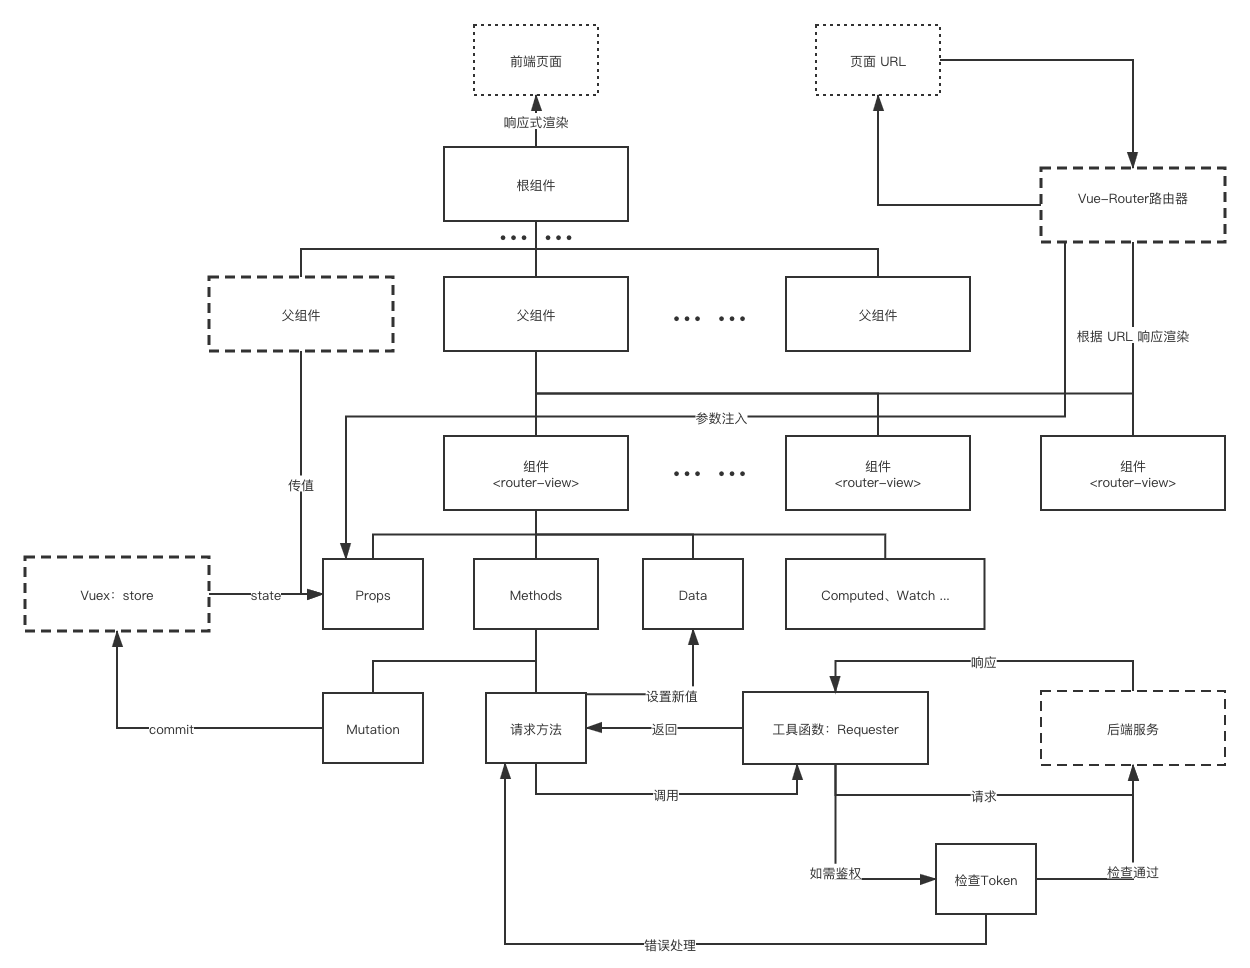
\includegraphics[width=\linewidth]{_images/前端模型.png}
    \caption{前端架构模型}
\end{figure}
Vue 的技术基础是将根节点组件挂载在页面的一个 DOM 元素上,而根节点组件由可由多个组件组成,如此向下细分成子组件。组件系统是 Vue 的另一个重要概念,因为它是一种抽象,允许我们使用小型、独立和通常可复用的组件构建大型应用。

组件的数据来源可以划分为:Props、Data、Computed。父子组件之间的数据通信通过 Props,而 Vue 的设计理念中,数据是自上而下单向流动。

面对需要多组件之间共享公共的数据的场景,需要引入 Vuex 的 store。store 将托管的公有数据 state,通过预先在根节点的注册,注入到需要的组件的 Props 中。如有需要对 store 中的数据进行修改,可以将 store 的 mutation 注入到组件的 Methods 中,通过提交(commit)mutation 实现对 store 中的 state 修改。

组件的 Data 也可能来自于用户的交互产生,又或是向后端服务请求的数据。组件中的请求方法,通过调用工具函数 Requester 向后端服务发起请求,其中如有必要应进行 Token 用户令牌的检查。响应得到的数据将返回给请求方法,进而给组件的 Data 赋予新值。

组件的渲染可能受控于父组件的逻辑,也可能受路由器的控制。在父组件中注册成为 <router-view> 的子组件,就通过 Vue-Router 的路由器,根据页面的 URL 动态响应渲染。其中也可以通过页面的 URL 动态路由匹配,向组件的 Props 注入匹配到的参数。


\subsubsection{后端架构模型}
\begin{figure}[htb]
    \centering
    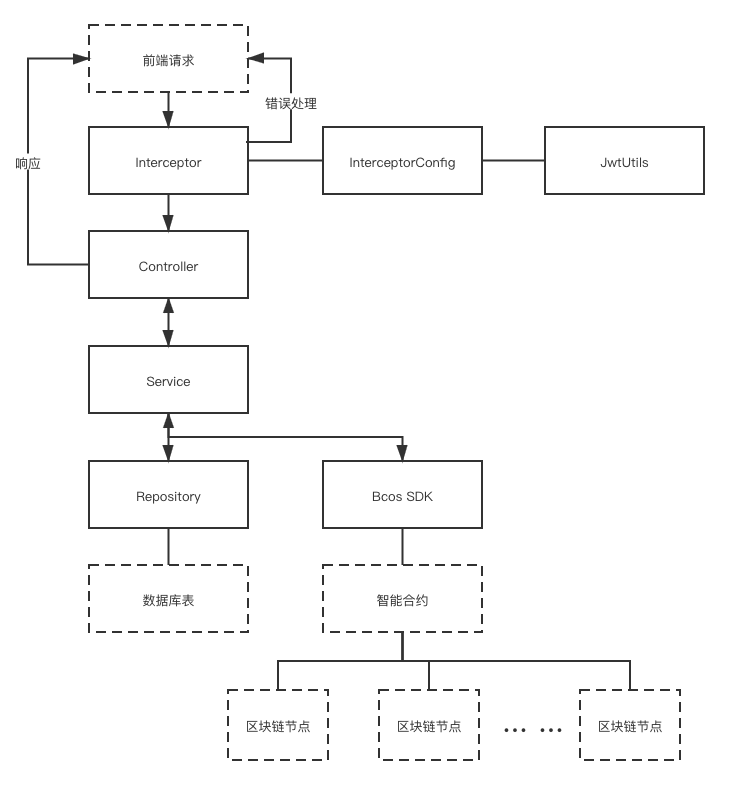
\includegraphics[width=0.85\linewidth]{_images/后端模型.png}
    \caption{后端架构模型}
\end{figure}
前端请求进入后端服务首先会被拦截器 Interceptor 所截获。通过 InterceptorConfig 配置需要拦截的 api 的 url 规则,并加入对应的 Interceptor。项目中的 JWT 鉴权流程便放在拦截器这一层运行。

请求根据具体 api 的 URL,进入不同的 controller,controller 根据业务调用对应的 Service 中的方法。由于使用了 SpringData JPA,数据库中的表与 Repository 对应且关联,因而 Service 中对 DAO 的操作则需要依赖于 Repository。

针对敏感数据需要上链的 Service,通过 Fisco Bcos 提供的 SDK,接入预先编译成 Java 文件的智能合约。而智能合约由通过密钥对的形式连接至区块链节点组成的网络。

\subsection{模块划分}
\begin{figure}[htb]
    \centering
    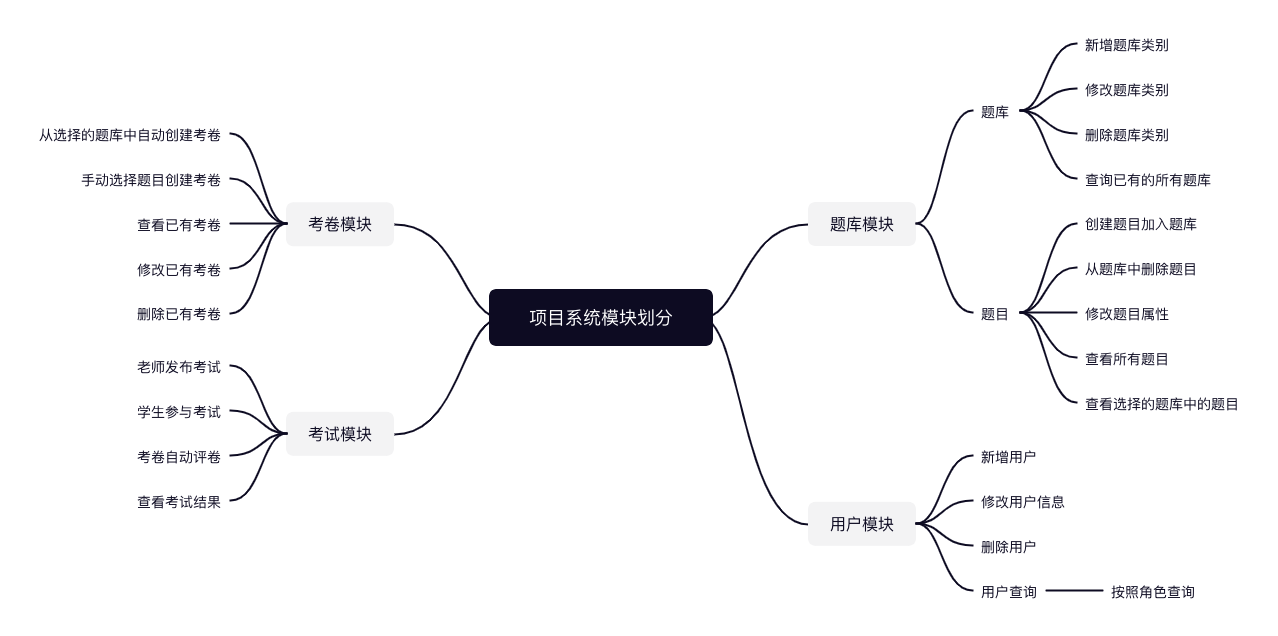
\includegraphics[width=\linewidth]{_images/功能模块划分.png}
    \caption{功能模块划分}
\end{figure}
项目系统根据功能划分成几个功能模块:题库模块、用户模块、考卷模块、考试模块。

按照权限分类用户角色,其对应的功能模块为:
\begin{itemize}
    \item 学生:考试模块
    \item 老师:题库模块、考试模块、考卷模块
    \item 管理员:题库模块、考试模块、考卷模块、用户模块
\end{itemize}

\subsection{Http 请求响应}
\subsubsection{前端请求}
\textit{front/Requester.js/post函数}
\begin{lstlisting}
function post(url, params = {}, needToken = true) {
    const {token} = TokenManager.getToken()
    ... ...
    Logger.log('request', {url, params})
    return axios({
        method: 'post',
        url: url,
        responseType: 'json',
        data: params,
        headers
    }).then(response => {
        const {data, status, statusText} = response
        Logger.log('response', data)
        return data
    }).catch(reason => {
        const {status, statusText} = reason.response
        Logger.error('response', status, statusText, reason.response)
        throw reason.response
    })
}
\end{lstlisting}